\chapter{User Guide}
This guide is for users of C4IAN who want to setup the environment and run the applications.
In this guide, we won't write about the modules themselves or their functions, we expect that you have read chapter \ref{ch:system-design} and \ref{ch:system-testing}.

This guide is divided into 2 sections:
\begin{itemize}[itemsep=1pt, topsep=5pt]
    \item Environment Setup: The dependencies and scripts that are needed to deploy the system.
    \item System Deployment: How to deploy each module (Router, Unit, CMD) in production.
    \item Usage: How to navigate the UI for both the CMD and Unit.
\end{itemize}

\section{Environment Setup}
You need to install the following packages on your system:
\begin{itemize}[itemsep=1pt, topsep=5pt]
    \item yarn
    \item NodeJS
    \item socat
    \item python3
    \item python3-pip
    \item a web browser (chrome, chromium or Firefox)
\end{itemize}

You may need to consult your system's manual on how to install them, because it differs from a distro to another.

The rest of this section assumes you are on a Debian derived OS.
If it's a different OS, you may need to edit the commands.

When you see \$ it means the command should be executed as a shell command.

\subsection{Golang 1.15.8}
\begin{verbatim}
$ sudo apt update && sudo apt install -y wget && (
    set -e
    cd /tmp
    wget -c https://golang.org/dl/go1.15.8.linux-amd64.tar.gz
    sudo tar xvf go1.15.8.linux-amd64.tar.gz
    sudo chown -R root:root ./go
    sudo mv ./go /usr/local
    mkdir -p $HOME/.config/go/1.15/{bin,pkg,src}
    echo >>"$HOME"/.bashrc
    echo 'export GOPATH="$HOME/.config/go/1.15"' >>"$HOME"/.bashrc
    echo 'export PATH="$PATH:/usr/local/go/bin:$GOPATH/bin"' >>"$HOME"/.bashrc
    echo >>"$HOME"/.bashrc
    . "$HOME"/.bashrc
)
\end{verbatim}

\subsection{python packages}
To install python packages, you should run:
\begin{verbatim}
$ sudo python3 -m pip install simple-websocket-server numpy watchgod
\end{verbatim}

\subsection{Libnetfilter-queue}
Needed for the router to get the packets from the kernel, it maybe installed on your system, here is how to get it:
\begin{verbatim}
$ sudo apt update && sudo apt install -y libnetfilter-queue-dev
\end{verbatim}

\subsection{Known Issues}
\subsubsection{Electron with libgconf}
\begin{verbatim}
electron: error while loading shared libraries: libgconf-2.so.4: cannot open shared object file: No such file or directory    
\end{verbatim}
\textbf{Solution} Run:
\begin{verbatim}
$ sudo apt install -y libgconf-2-4
\end{verbatim}

\subsubsection{Writing to \texttt{/tmp/}}
On some systems, writing to \texttt{/tmp/} directory may be disabled, we need to write to it for many different reasons.
So if some script complained that there are no permissions to write to /tmp/ you may need to execute the folowing command:
\begin{verbatim}
$ sudo sysctl fs.protected_regular=0
\end{verbatim}

\section{System Deployment}
This section is divided into 3 subsections on how to deploy:
\begin{itemize}[itemsep=1pt, topsep=5pt]
    \item The Router.
    \item Unit.
    \item CMD.
\end{itemize}

You need to execute all the next commands in \texttt{src/} directory.

Before running any program you need to build them all, run:
\begin{verbatim}
$ make apps router
\end{verbatim}

\subsubsection{Router Deployment}
Router is deployed on all devices that should communicate within an adhoc network, whether its unit or cmd device.

To enter adhoc mode and run the router locally assuming interface=wlan0 and ip=10.0.0.1
\begin{verbatim}
$ sudo ./start local router -- wlan0 10.0.0.1
\end{verbatim}

or to override default env variables assuming password is \texttt{somePass} and the \texttt{SSID} you want to use is \texttt{someSSIDName}:
\begin{verbatim}
$ sudo PASS=somePass SSID=someSSIDName ./start local router -- wlan0 10.0.0.1
\end{verbatim}

You may need to pass more options to the router to control it more. 
To get a list of router's arguments:
\begin{verbatim}
$ ./router/router --help
\end{verbatim}

\subsubsection{Unit Deployment}
Unit is only deployed on unit devices alongside the router.

You might need to develop a \texttt{HAL} program that interfaces with the unit daemon.
The interface for HAL is at \texttt{src/unit/halapi} with an example implementation (for testing on emulation) in \texttt{src/unit/halsimulation}.

To deploy the unit daemon locally, simply run:
\begin{verbatim}
$ sudo ./start local unit
\end{verbatim}

You may need to pass more options to the unit daemon to control it more. 
To get a list of units's arguments:
\begin{verbatim}
$ ./unit/daemon/daemon --help
\end{verbatim}

\subsubsection{Command-Center Daemon Deployment}
Command-Center is only deployed on command center computers alongside the router.

To deploy the cmd daemon locally, simply run:
\begin{verbatim}
$ sudo ./start local cmd
\end{verbatim}

You may need to pass more options to the cmd daemon to control it more. 
To get a list of units's arguments:
\begin{verbatim}
$ ./cmd/daemon/daemon --help
\end{verbatim}

\subsubsection{Command-Center UI Deployment}
One command center daemon may be connected to multiple UI processes.
They could be deployed from multiple computers.

To run the cmd UI locally, run:
\begin{verbatim}
$ cd cmd/ui && yarn && yarn run electron
\end{verbatim}

\section{Usage}
\label{sec:usage}
This section describes how to use the system modules.

\subsection{Router}
For the router, no changes should be made on the system to use it.
Every program shall proceed as normal with opening TCP/UDP sockets and communicating with the outside world as usual.
Note that the router doesn't route Unix sockets traffic, only TCP/UDP/ICMP over IPv4.

\subsection{Unit}
It depends on what HW you are building.
If you used the unit UI, it just functions as the cmd UI, which we will describe in the subsection \ref{subsec:cmdui-usage}.
If you used the halsimulation, it just sends commands and messages, and you don't interact with it.

\subsection{Command Center UI} 
\label{subsec:cmdui-usage}

As shown in Figure \ref{fig:cmd-ui-port} You should have a window with the UI asking you about the port of the daemon, to get it consult the logs of the running cmd daemon.

\begin{figure}[!htb]
    \centering
    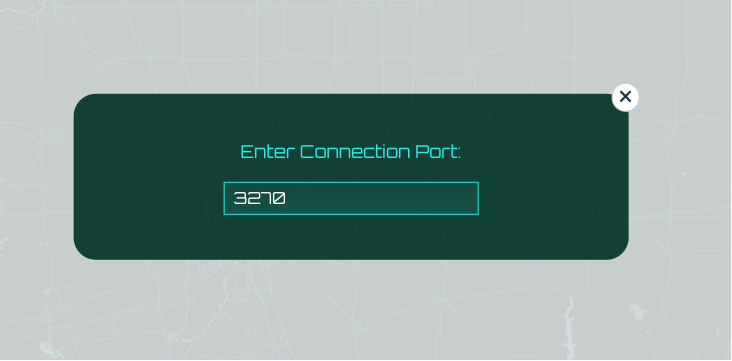
\includegraphics[width=11cm]{images/cmd-ui-port.png}
    \caption{CMD UI Filling Port Number}
    \label{fig:cmd-ui-port}
\end{figure}

\begin{figure}[!htb]
    \centering
    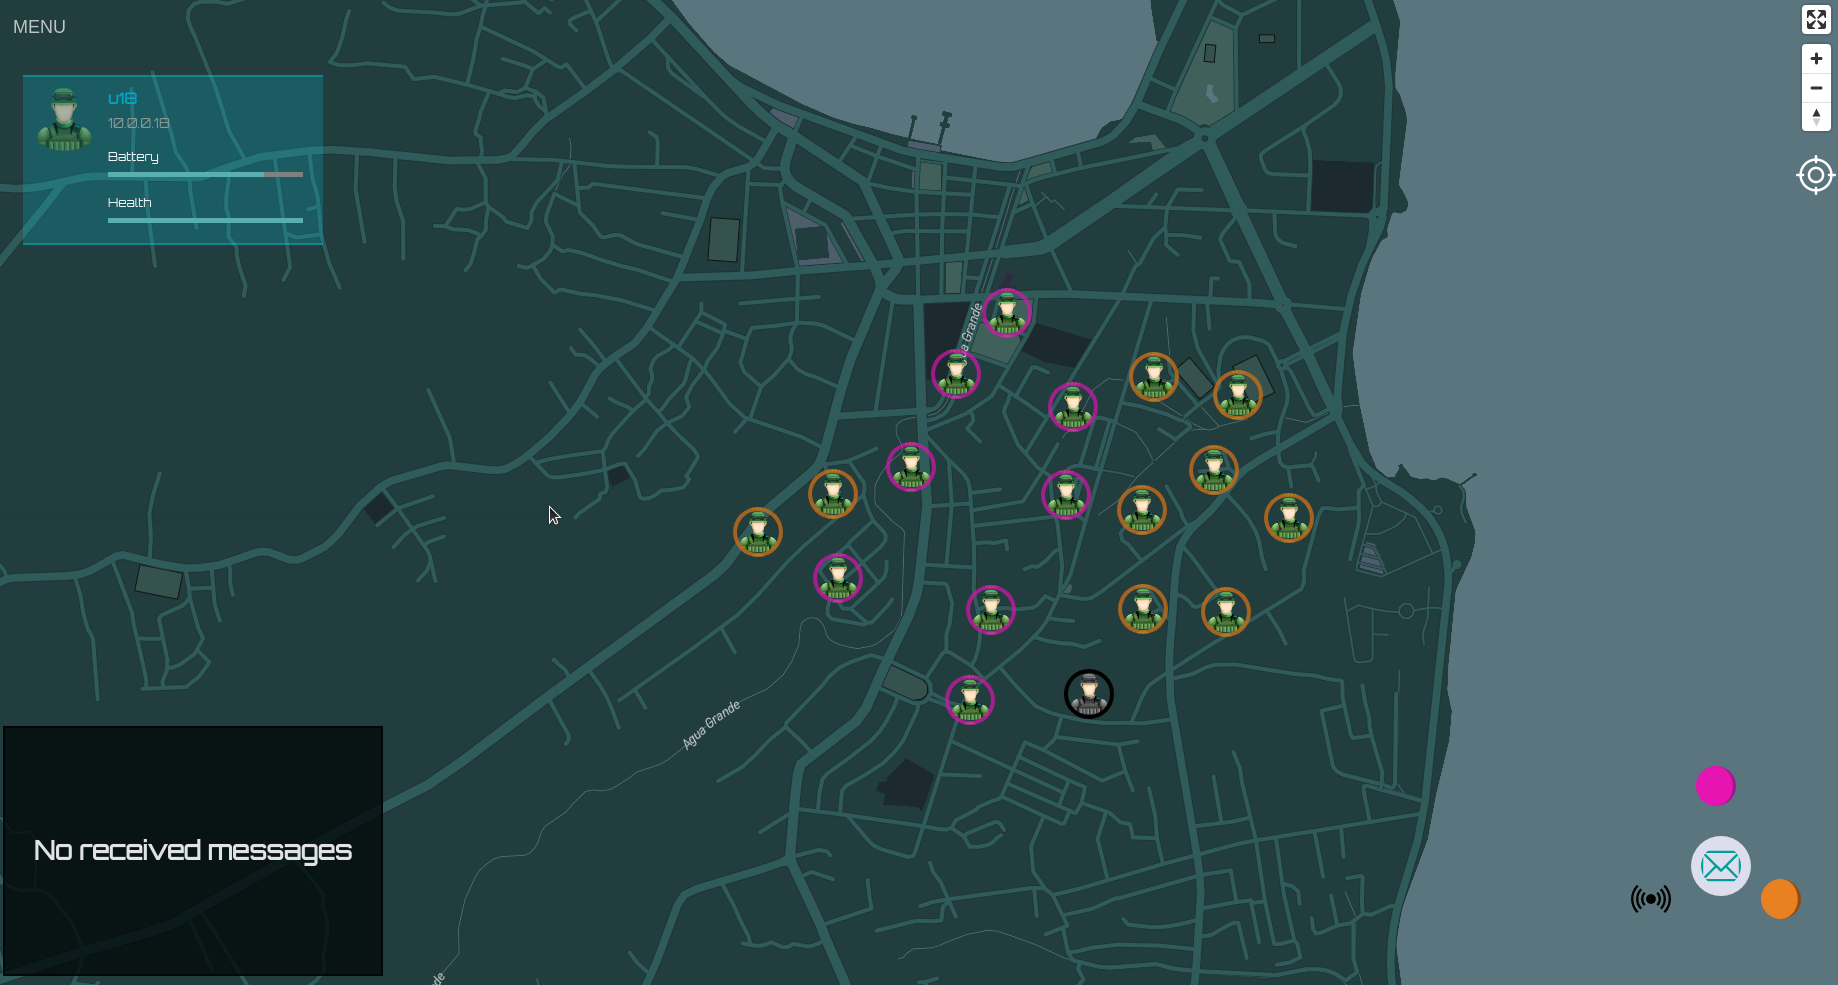
\includegraphics[width=\linewidth]{images/cmd-ui-map.png}
    \caption{CMD UI Map Page}
    \label{fig:cmd-ui-map}
\end{figure}

\begin{figure}[!htb]
    \centering
    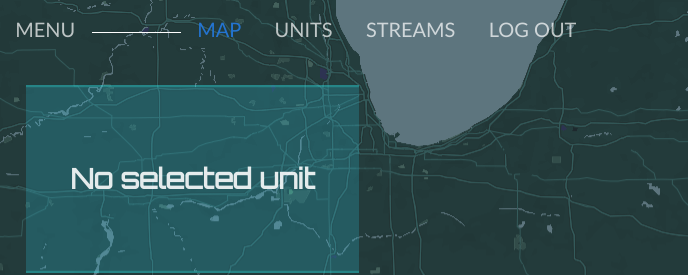
\includegraphics[width=\linewidth]{images/cmd-ui-menu.png}
    \caption{CMD UI Menu}
    \label{fig:cmd-ui-menu}
\end{figure}

\begin{figure}[!htb]
    \centering
    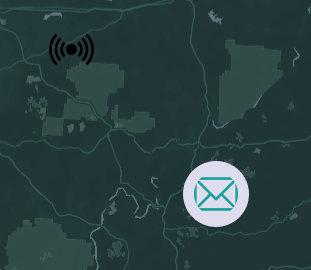
\includegraphics[width=11cm]{images/cmd-ui-bcast-button.png}
    \caption{CMD UI Broadcast Button}
    \label{fig:cmd-ui-bcast-button}
\end{figure}

\begin{figure}[!htb]
    \centering
    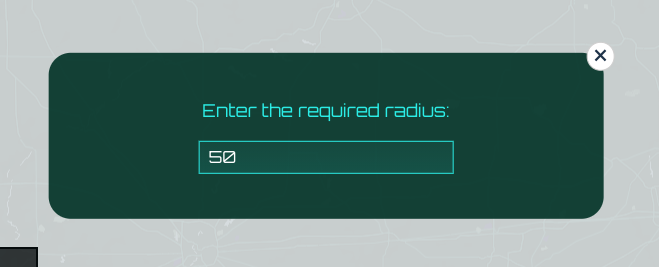
\includegraphics[width=11cm]{images/cmd-ui-bcast-dialog.png}
    \caption{CMD UI Broadcast Dialog}
    \label{fig:cmd-ui-bcast-dialog}
\end{figure}

After setting the port, you will be directed to the home page (Figure \ref{fig:cmd-ui-map}) which shows a map of units and a menu (Figure \ref{fig:cmd-ui-menu}) and a floating button if clicked shows the button for broadcasting a message (Figure \ref{fig:cmd-ui-bcast-button} and Figure \ref{fig:cmd-ui-bcast-dialog}.)

Clicking on the \textit{Units} from menu button directs to the units page, which contains the list of units and videos and audios and code messages, as shown in Figure \ref{fig:cmd-ui-units}.

\begin{figure}[!htb]
    \centering
    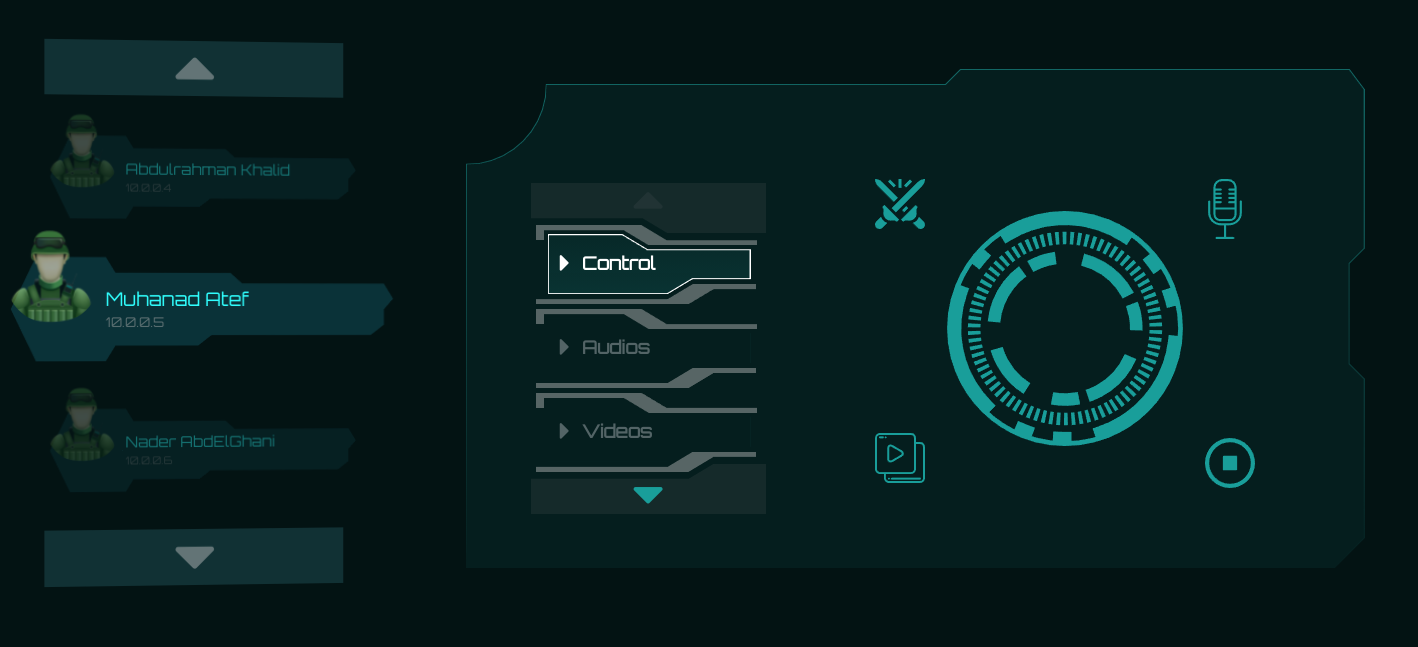
\includegraphics[width=11cm]{images/cmd-ui-units.png}
    \caption{CMD UI Units Page}
    \label{fig:cmd-ui-units}
\end{figure}

Figure \ref{fig:cmd-ui-code-msg} shows how to send a code message by clicking on one of the icons, each has its code, which will be sent to the selected unit.

\begin{figure}[!htb]
    \centering
    
\includegraphics[width=0.6\linewidth]{images/cmd-ui-code-msg.png}
    \caption{CMD UI Code Message (Attack)}
    \label{fig:cmd-ui-code-msg}
\end{figure}

You may send a video streaming request to the unit, as shown in Figure \ref{fig:cmd-ui-req-video}.
And then you need to go to the streaming page, from the menu button, as show in Figure \ref{fig:cmd-ui-streaming}, which takes you to a page showing the video streaming live from the unit's video sources with the captured audio (if any).

\begin{figure}[!htb]
    \centering
    
\includegraphics[width=0.6\linewidth]{images/cmd-ui-req-video.png}
    \caption{CMD UI Requesting Video Streaming From Unit}
    \label{fig:cmd-ui-req-video}
\end{figure}

\begin{figure}[!htb]
    \centering
    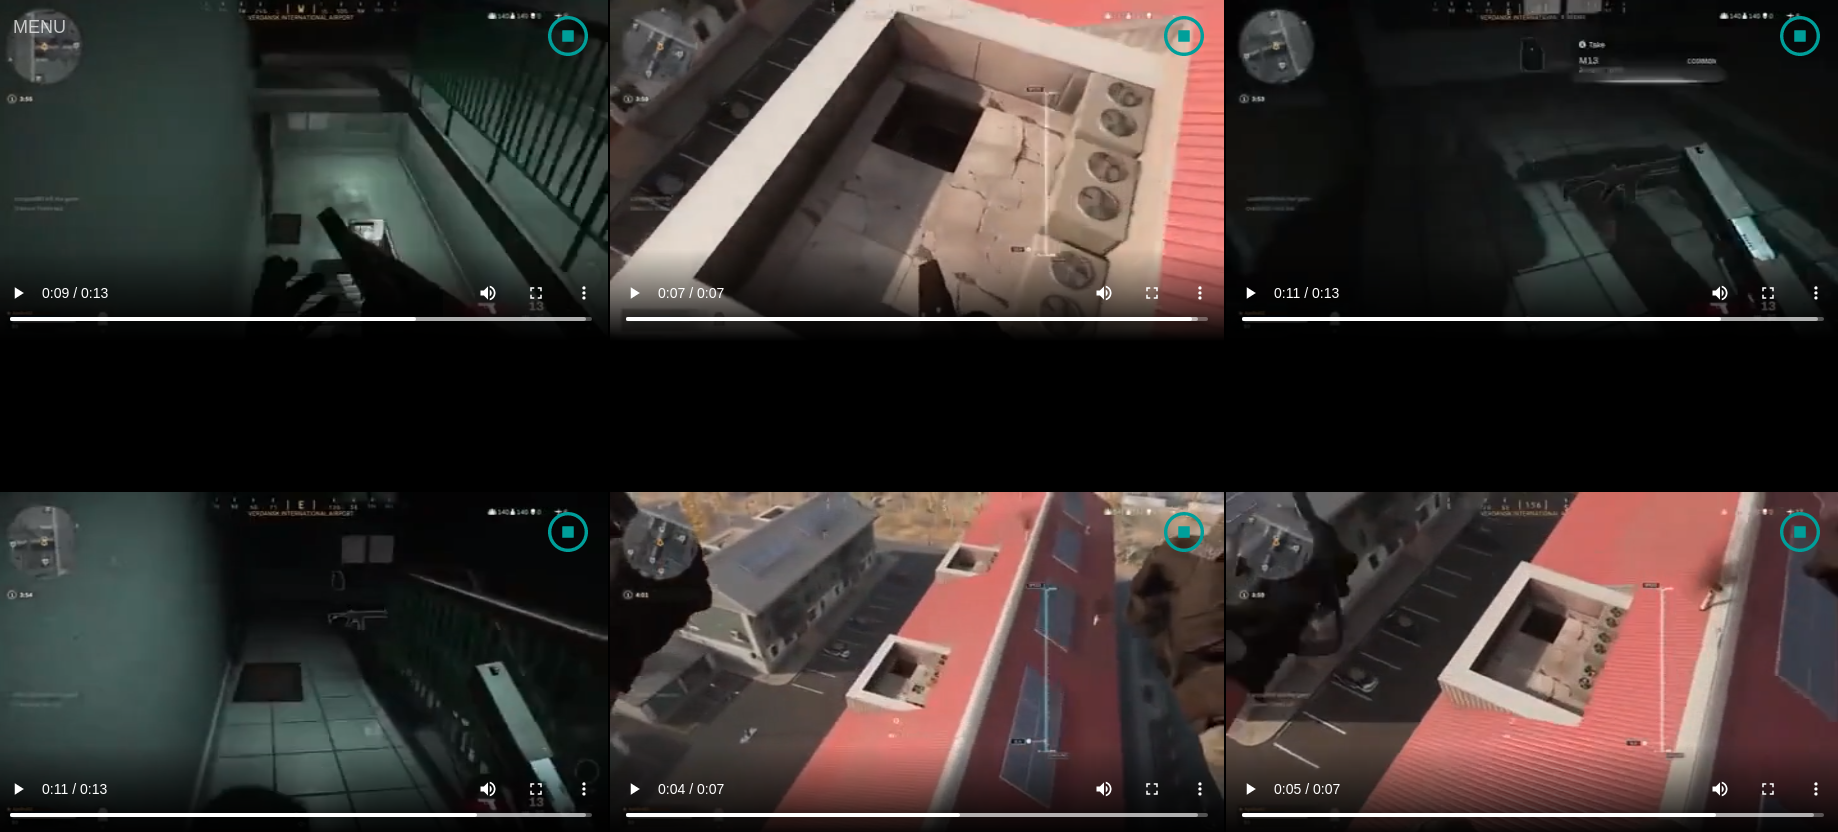
\includegraphics[width=16cm]{images/cmd-ui-streaming.png}
    \caption{CMD UI Streaming Page}
    \label{fig:cmd-ui-streaming}
\end{figure}
